% !TEX program = xelatex
\documentclass[]{article}
\usepackage{commons/course}

\begin{document}
\printheader

\section{}
\subsection{}
یکی از کار‌هایی که می‌توان کرد این است یک تبادل کلید دیفی هلمن انجام گیرد به صورتی که تمامی
پارامتر‌ها با کلید
$K_{c,s}$
امضا شوند. (مثلا به کمک الگوریتم \lr{CBC-MAC}) با این کار تنها
$C$ و $V$
و
$KDC$
می‌توانند که پارامتر‌ها را امضا کنند و از انجا که
$KDC$
نمی‌تواند ترافیکی را عوض کند می‌دانیم که حمله‌ی مرد میانی نمی‌تواند رخ دهد و کلید جدید
$K'$
صرفا بین دو
$C$ و $V$
ساخته می‌شود و فقط این دو کلید را دارند.
\subsection{}
همان طور که در قسمت قبل هم گفته شد در این صورت حمله مرد میانی می‌تواند صورت بگیرد چرا که خود
$KDC$
می‌تواند که پارامتر‌ها را امضا بکند.
\subsection{}
به نظر من یکی از کار‌های نسبتا ساده‌ای که می‌توان انجام داد این است که یکی از طرفین کلید تصادفی
$K'$
را تولید کند و سپس آن را در ابتدا با
$K_{c,s,1}$ و در ادامه با $K_{c,s,2}$
رمز می‌کند. در این حالت در صورتی که
$KDC1$
بخواهد که رمز را باز کند نیاز دارد که کلید
$KDC2$
را بداند و در صورتی که
$KDC2$
بخواهد رمز را باز کند باید کلید
$KDC1$
را بداند. از انجا که فرض کردیم تبانی نداریم پس این کار را نمی‌توانند انجام دهند.
در نهایت نیز برای صحت ارسال می‌توان هم با
$K_{c,s,1}$ و هم $K_{c,s,2}$
کلید را امضا کرد و سپس آن را رمز کرد.
\section{}
\subsection{}
برای ساخت کلید من از
\link{https://irtfweb.ifa.hawaii.edu/~lockhart/gpg/}{این}
لینک استفاده کردم. همان طور که مشخص است در ابتدا از دستور
\LRE{\verb|gpg --gen-key|}
استفاده می‌کنیم. در ادامه تمامی موارد خواسته شده را وارد می‌کنیم و یک پسورد برای کلید خود انتخاب می‌کنیم.
نتیجه دستور در شکل
\ref{fig:gpg:keygen}
موجود است.
\begin{figure}[H]
    \centering
    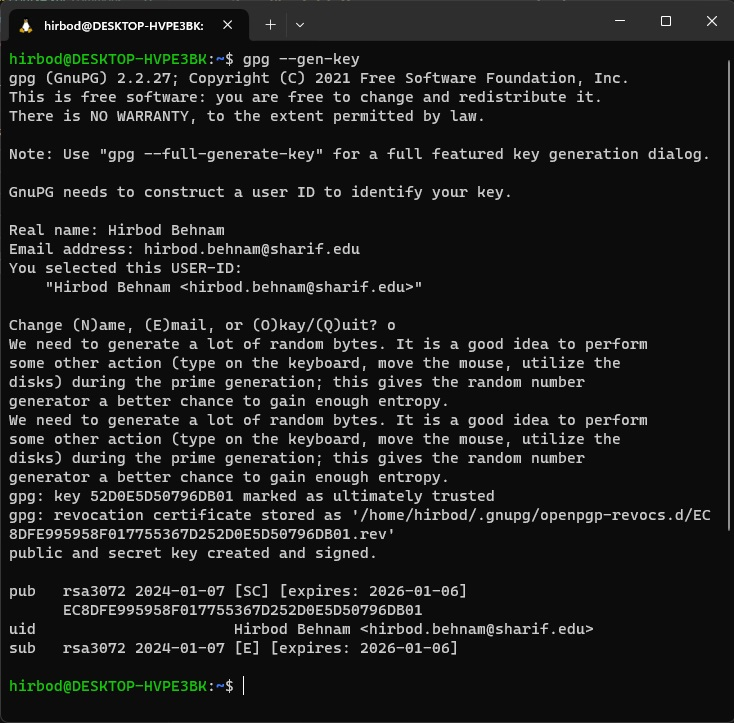
\includegraphics[scale=0.5]{pics/gpg-keygen.jpg}
    \caption{ساخت \lr{GPG key}}
    \label{fig:gpg:keygen}
\end{figure}
حال می‌توانیم با دستور
\LRE{\verb|gpg --list|}
تمامی کلید‌های خود را مشاهده کنیم. همچنین می‌توان با دستور زیر کلید عمومی مربوط به دانشگاه را استخراج کرد.
\begin{latin}
\begin{lstlisting}[language=sh]
gpg --export -a "hirbod.behnam@sharif.edu"
\end{lstlisting}
\end{latin}
نتیجه این دستورات را می‌توانید در شکل
\ref{fig:gpg:view}
ببینید.
\begin{figure}[H]
    \centering
    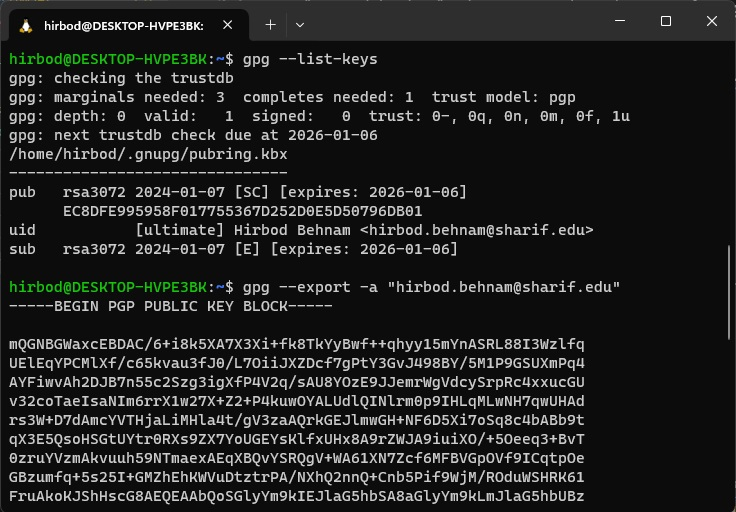
\includegraphics[scale=0.5]{pics/gpg-view.jpg}
    \caption{مشاهده کلید‌های PGP}
    \label{fig:gpg:view}
\end{figure}
\subsection{}
در این قسمت در ابتدا نیاز است که کلید عمومی داده شده را
import
کنیم. برای این کار از دستور زیر استفاده می‌کنیم. نتیجه‌ی آن در عکس
\ref{fig:gpg:import}
آمده است.
\begin{latin}
\begin{lstlisting}[language=sh]
gpg --import Reza_0xCFBEEE88_public.asc
\end{lstlisting}
\end{latin}
\begin{figure}[H]
    \centering
    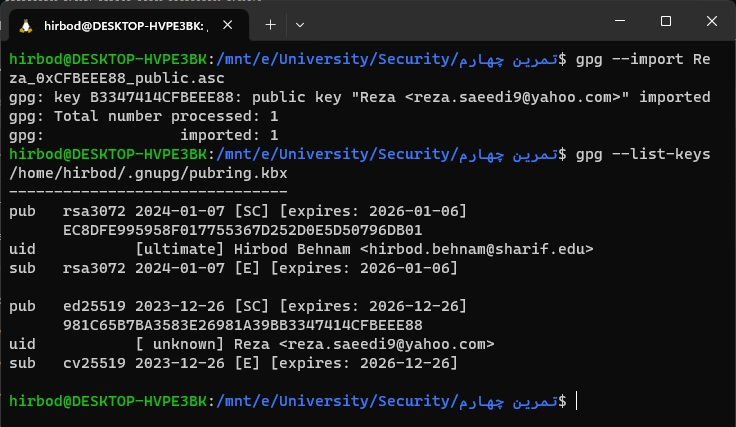
\includegraphics[scale=0.5]{pics/gpg-import.jpg}
    \caption{اضافه کردن کلید PGP طراح تمرین به GPG}
    \label{fig:gpg:import}
\end{figure}
حال باید دیتایی را در ابتدا امضا و سپس رمزنگاری کنیم. برای این کار از دستور زیر استفاده می‌کنیم.
دقت کنید که این دستور یک فایل را رمزنگاری و امضا می‌کند. در نتیجه کافی است که صرفا متن ایمیل را در فایلی
بنویسیم و آن فایل را رمز کنیم.
(\link{https://medium.com/@acparas/how-to-encrypt-and-sign-a-file-with-gpg-531070b2fa6d}{منبع})
\begin{latin}
\begin{lstlisting}[language=sh]
    gpg --output email.pgp --armor --encrypt --sign --recipient reza.saeedi9@yahoo.com email-plaintext.txt
\end{lstlisting}
\end{latin}
همان طور که مشاهده می‌کنید محتوای فایل تولید شده رمزگذاری شده است.
\begin{figure}[H]
    \centering
    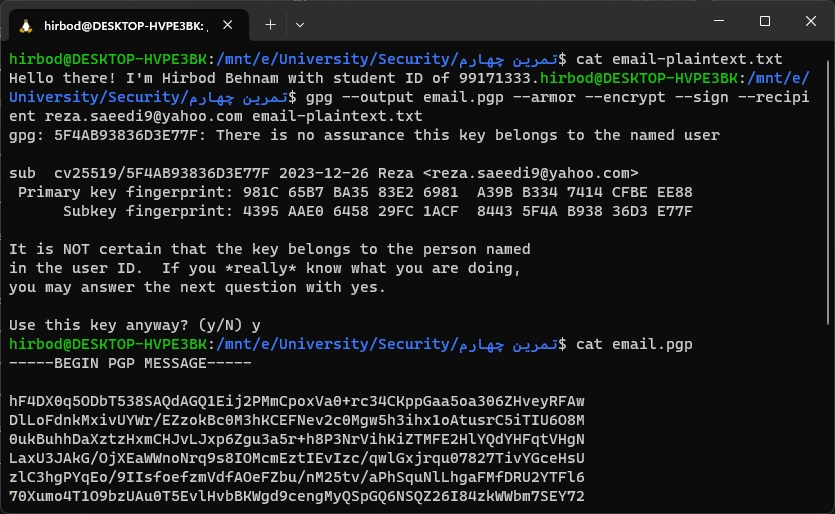
\includegraphics[scale=0.5]{pics/gpg-encrypt.jpg}
    \caption{رمزنگاری پیام}
    \label{fig:gpg:encrypt}
\end{figure}
در نهایت نیز محتوای این فایل را ایمیل کردم. دقت کنید که در کل مراحل بالا
\LRE{\verb|--armor|}
برای این بود که نتیجه به صورت اسکی کد باشد و بتوان آن را کپی و پیست در ایمیل کرد.
ایمیل فرستاده شده نیز در شکل
\ref{fig:gpg:email}
قابل مشاهده است.
\begin{figure}[H]
    \centering
    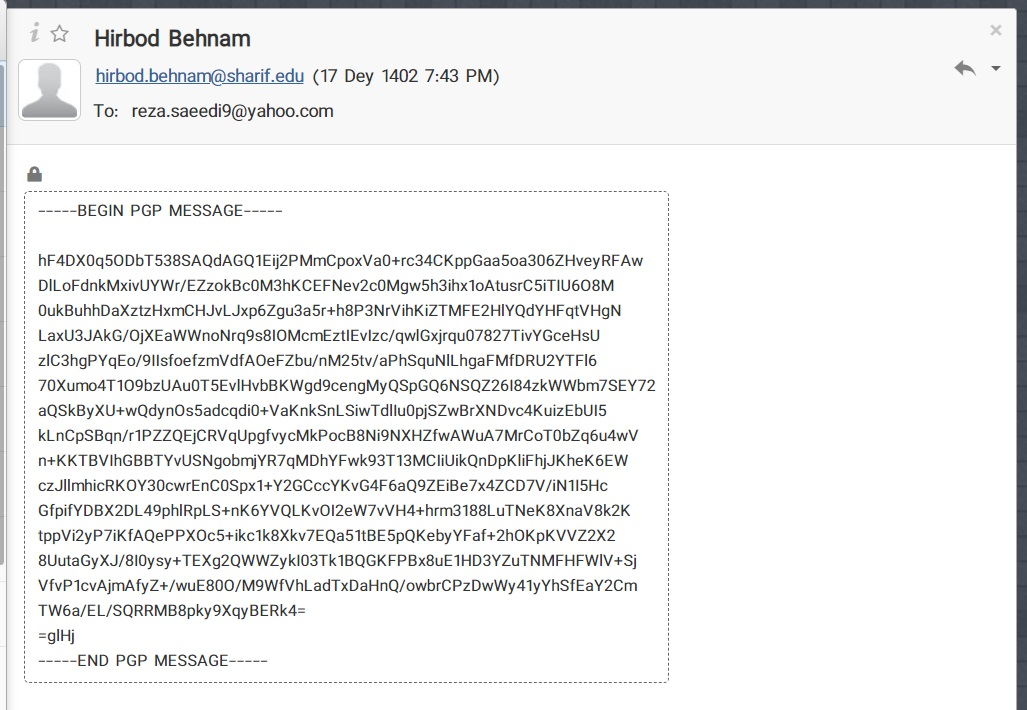
\includegraphics[scale=0.35]{pics/gpg-email.jpg}
    \caption{ایمیل فرستاده شده}
    \label{fig:gpg:email}
\end{figure}
\section{}
\subsection{}
\begin{itemize}
    \item \textbf{\lr{Bruteforce Attack}}: این حمله عملا سعی می‌کند که با حدس زدن کلید رمزنگاری رمزنگاری را بشکاند. به صورت صریح این مورد در درس ذکر نشده است اما من فکر می‌کنم که به صورت کلی نمی‌توان جلوی \lr{bruteforce} را گرفت اما می‌توان احتمال آن را کم کرد. به عنوان مثال می‌توان از الگوریتم‌های رمزنگاری قوی استفاده کرد.
    \item \textbf{\lr{Known Plaintext Attack}}: در این حمله مهاجم هم یک متن به صورت رمزگشایی شده را دارد و هم یک متن به صورت رمزشده را دارد. این نوع حمله نیز به کمک \lr{cipher} استفاده شده می‌تواند بی اثر شود.
    \item \textbf{\lr{Reply Attack}}: این حمله بدین صورت است که مهاجم یکی از پکت‌های قبلی کاربر را بدون تغییر به سرور می‌فرستد. این حمله به کمک استفاده از \lr{sequence number} و \lr{window} قابل جلوگیری است چرا که پیام‌هایی که در قبل دریافت شده‌اند را داریم و در صورت مشاهده‌ی یک پیام تکراری آن را دور می‌ریزیم.
    \item \textbf{\lr{Password Sniffing}}:
    \item \textbf{\lr{IP Spoofing}}: این حمله بدین صورت است که پکت‌هایی درست می‌کنیم که IP مبدا را عوض می‌کنیم و چیزی به غیر از آی‌پی واقعی خود قرار می‌دهیم. (\link{https://en.wikipedia.org/wiki/IP_address_spoofing}{منبع})
    \item \textbf{\lr{IP Hijacking}}: این نوع حملات بدین صورت هستند که واقعا \lr{IP}هایی را در شبکه در اختیار می‌گیریم که برای ما نیست و دیتا‌هایی که برای ما نباید بیاید برای ما می‌آید.  (\link{https://www.oreilly.com/library/view/hackers-beware/0735710090/0735710090_ch05lev1sec1.html}{منبع})
    \item \textbf{\lr{SYN Flooding}}: در این نوع حمله یک مهجام یک عالمه پکت \lr{SYN} که اولین پکت برای شروع یک کانکشن TCP است را برای یک سرور به تعداد زیادی می‌فرستد به طوری که IP مبدا آن برای شخص دیگر باشد. (\link{https://www.cloudflare.com/learning/ddos/syn-flood-ddos-attack/}{منبع})
\end{itemize}
\subsection{}
در این قسمت من از دو ماشین مجازی
\lr{Ubuntu 22.04}
استفاده کردم که به یک اداپتور
\lr{host only}
در
\lr{Virtualbox}
وصل بودند. با این کار می‌توان که از هر کدام از ماشین مجازی‌ها دیگری را پینگ کرد.
\section{}
\section{}
\begin{enumerate}
    \item \link{https://superuser.com/a/634471}{منبع} \begin{latin}
\begin{lstlisting}[language=sh]
iptables -A OUTPUT -j ACCEPT
\end{lstlisting}
    \end{latin}
    \item \link{https://www.digitalocean.com/community/tutorials/iptables-essentials-common-firewall-rules-and-commands\#allowing-established-and-related-incoming-connections}{منبع 1} \link{https://www.ipserverone.info/knowledge-base/how-to-open-ports-in-iptables}{منبع 2} \begin{latin}
\begin{lstlisting}[language=sh]
iptables -A INPUT -j DROP
iptables -A INPUT -m conntrack --ctstate ESTABLISHED -j ACCEPT
iptables -I INPUT -p tcp --dport 22 -j ACCEPT
\end{lstlisting}
\end{latin}
    \item \link{https://www.cyberciti.biz/tips/linux-iptables-9-allow-icmp-ping.html}{منبع} \begin{latin}
\begin{lstlisting}[language=sh]
iptables -A INPUT -p icmp -j ACCEPT
iptables -A INPUT -p icmp --icmp-type redirect -j DROP
\end{lstlisting}
    \end{latin}
    \item برای این قسمت در ابتدا باید قابلیت \lr{IP forwarding} را در لینوکس فعال کنیم. برای این کار کافی است که از دستور زیر استفاده کنیم: \begin{latin}
\begin{lstlisting}[language=sh]
echo "net.ipv4.ip_forward=1" >> /etc/sysctl.conf
\end{lstlisting}
\end{latin}
    سپس در ادامه باید دستگاه را یک بار ری استارت کنیم. در نهایت نیز از دستورات زیر استفاده می‌کنیم: \link{https://unix.stackexchange.com/a/585613}{منبع}
\begin{latin}
\begin{lstlisting}[language=sh]
iptables -t nat -A PREROUTING -p tcp --dport 8080 -j DNAT --to-destination 127.0.0.1:80
iptables -t nat -A POSTROUTING -j MASQUERADE
\end{lstlisting}
\end{latin}
    \item برای این سوال من در گوگل صرفا سرچ کردم که چه قوانینی برای iptables و مقابله با DDOS خوب هستند که به
    \link{https://gist.github.com/mattia-beta/bd5b1c68e3d51db933181d8a3dc0ba64}{این لینک}
    رسیدم. از بین دستوراتی که در این لینک موجود بود برخی از آن‌ها که به نظرم تاثیرات خیلی خوب می‌توانست بگذارد را
    برداشتم و آن‌ها را در ادامه لیست کردم.
\begin{latin}
\begin{lstlisting}[language=sh]
# Drop invalid packets
iptables -t mangle -A PREROUTING -m conntrack --ctstate INVALID -j DROP
   
# Drop TCP packets that are new and are not SYN
/sbin/iptables -t mangle -A PREROUTING -p tcp ! --syn -m conntrack --ctstate NEW -j DROP

# Block packets with bogus TCP flags
iptables -t mangle -A PREROUTING -p tcp --tcp-flags FIN,SYN,RST,PSH,ACK,URG NONE -j DROP
iptables -t mangle -A PREROUTING -p tcp --tcp-flags FIN,SYN FIN,SYN -j DROP
iptables -t mangle -A PREROUTING -p tcp --tcp-flags SYN,RST SYN,RST -j DROP
iptables -t mangle -A PREROUTING -p tcp --tcp-flags SYN,FIN SYN,FIN -j DROP
iptables -t mangle -A PREROUTING -p tcp --tcp-flags FIN,RST FIN,RST -j DROP
iptables -t mangle -A PREROUTING -p tcp --tcp-flags FIN,ACK FIN -j DROP
iptables -t mangle -A PREROUTING -p tcp --tcp-flags ACK,URG URG -j DROP
iptables -t mangle -A PREROUTING -p tcp --tcp-flags ACK,FIN FIN -j DROP
iptables -t mangle -A PREROUTING -p tcp --tcp-flags ACK,PSH PSH -j DROP
iptables -t mangle -A PREROUTING -p tcp --tcp-flags ALL ALL -j DROP
iptables -t mangle -A PREROUTING -p tcp --tcp-flags ALL NONE -j DROP
iptables -t mangle -A PREROUTING -p tcp --tcp-flags ALL FIN,PSH,URG -j DROP
iptables -t mangle -A PREROUTING -p tcp --tcp-flags ALL SYN,FIN,PSH,URG -j DROP
iptables -t mangle -A PREROUTING -p tcp --tcp-flags ALL SYN,RST,ACK,FIN,URG -j DROP

# Limit connections per source IP
iptables -A INPUT -p tcp -m connlimit --connlimit-above 111 -j REJECT --reject-with tcp-reset

# Limit new TCP connections per second per source IP
iptables -A INPUT -p tcp -m conntrack --ctstate NEW -m limit --limit 60/s --limit-burst 20 -j ACCEPT
iptables -A INPUT -p tcp -m conntrack --ctstate NEW -j DROP
\end{lstlisting}
\end{latin}
    کاری که این دستورات می‌کنند این است که در ابتدا پکت‌هایی که اصلا شکل درستی ندارند (یعنی هیچ پروتکل \lr{TCP-UDP-ICMP}) نیستند
    را دراپ می‌کنیم. در ادامه جلوی پکت‌های TCP را می‌گیریم که به هیچ کانکشنی در سیستم‌عامل مپ نشده‌اند. بدین معنا که مثلا ممکن است مهاجمی
    یک پکت FIN برای یک کانکشنی بفرستد که وجود ندارد.
    در ادامه جلوی پکت‌های TCP را می‌گیریم که فلگ‌های آن‌ها ممکن نیست که حالت‌های خاصی داشته باشند. به عنوان مثال
    هیچ گاه یک پکت نمی‌توان SYN و FIN همزمان داشته باشد!
    در آخر که به نظر من مهم ترین کاری است که می‌توان انجام داد این است که تعداد کانکشن‌های TCP
    از یک IP را محدود کنیم. در اینجا به کاربران با یک IP اجزاه داده نمی‌شود که همزمان 111 و یا بیشتر کانکشن باز داشته باشند.
    در نهایت نیز سرعت باز کردن کانشکن‌های جدید را محدود می‌کنیم.
\end{enumerate}
\end{document}
